\def\year{2017}\relax
%File: formatting-instruction.tex
\documentclass[letterpaper]{article}

\usepackage{graphicx}
\usepackage{amsmath}
\usepackage{amssymb}
\usepackage{amsthm,mathrsfs,amsfonts,dsfont}
\usepackage{algorithm}
\usepackage{algorithmic}
\usepackage{threeparttable}
\usepackage{multirow}
\usepackage{subfigure}
\usepackage{color}
\usepackage{epstopdf}
\usepackage{bm}
%\usepackage[vlined,boxed,ruled]{algorithm2e}
\usepackage{url}
\usepackage{xspace}

\newtheorem{corollary}{Corollary}
\newtheorem{definition}{Definition}
\newtheorem{theorem}{Theorem}
\newtheorem{proposition}{Proposition}
\newtheorem{lemma}{Lemma}
\newtheorem{remark}{Remark}



\usepackage{aaai17}
\usepackage{times}
\usepackage{helvet}
\usepackage{courier}



\def\bD{{\bf D}}
\def\bI{{\bf I}}
\def\bE{{\bf E}}
\def\blambda{{\bm \lambda}}
\def\calL{{\mathcal{L}}}
\def\calC{{\mathcal{C}}}
\def\calS{{\mathcal{S}}}
\def\calF{{\mathcal{F}}}
\def\bL{{\bf L}}
\def\bO{{\bf O}}
\def\bU{{\bf U}}
\def\bV{{\bf V}}
\def\dsR{\mathds{R}}
\def\bX{{\bf X}}
\def\bx{{\bf x}}
\def\btx{{\tilde{\bf x}}}
\def\by{{\bf y}}
\def\bw{{\bf w}}
\def\btw{{\tilde{\bf w}}}
\def\tK{\tilde{K}}
\def\txi{\tilde{\xi}}
\def\tildeb{{\tilde{b}}}
\def\tphi{{\tilde{\phi}}}
\def\bz{{\bf z}}
\def\br{{\bf r}}
\def\bv{{\bf v}}
\def\bb{{\bf b}}
\def\bp{{\bf p}}
\def\bA{{\bf A}}
\def\bI{{\bf I}}

\def\bx{{\bf x}}
\def\bX{{\bf X}}
\def\by{{\bf y}}
\def\bY{{\bf Y}}
\def\bw{{\bf w}}
\def\bW{{\bf W}}
\def\balpha{{\bm \alpha}}
\def\bmu{{\bm \mu}}
\def\bK{{\bf K}}
\def\bg{{\bf g}}
\def\bp{{\bf p}}
\def\p{p}
\def\bP{{\bf P}}

\def\balpha{{\bm \alpha}}
\def\bbeta{{\bm \beta}}
\def\eg{{\emph{e.g.}}}
\def\zerocolumn{{\bf 0}}

\def\ttTP{{\tt TP}}
\def\ttFP{{\tt FP}}
\def\ttFN{{\tt FN}}

\def\st{{\text{s.t.}}}
\def\rank{{\text{rank}}}
\def\Tr{{\text{Tr}}}

\def\yanred{\textcolor{red}}
\def\yanblue{\textcolor{blue}}


\frenchspacing
\setlength{\pdfpagewidth}{8.5in}
\setlength{\pdfpageheight}{11in}
\pdfinfo{
/Title (Insert Your Title Here)
/Author (Put All Your Authors Here, Separated by Commas)}
\setcounter{secnumdepth}{0}
 \begin{document}


% The file aaai.sty is the style file for AAAI Press
% proceedings, working notes, and technical reports.
%



\title{Outlier Reject for Late Fusion on Visual Recognition}

%\author{AAAI Press\\
%Association for the Advancement of Artificial Intelligence\\
%2275 East Bayshore Road, Suite 160\\
%Palo Alto, California 94303\\
%}



\maketitle



\begin{abstract}
% First: A big picture of the scenario which we would consider
In many real world applications, data can be represented in multiple ways/features, which would describe various characteristics of data.
Many works have shown that it could often improve the performance to make use of these features together.
% Second: what BIG problem would we like to solve?
Late fusion, which combines the predictions of multiple features, is a commonly used approach to generate the final decision for a test instance.
% Third: specify the detailed problem: find a precise position for our paper
However, it is ubiquitous that different features would dispute on some data, leading to the requirement of outlier rejection for late fusion algorithms.
% Fourth: general introduction of our method
In this paper, we propose an efficient matrix factorization based approach to fuse predictions from multiple sources, which could
relieve the performance degeneration caused by the controversy of multiple features on test data.
% Some unvalued sentence(s)
Extensive experiments demonstrate that the proposed method is effective to remove outliers and improve fusion performance.
% Written by DXY:
%We formulate the late score fusion algorithm as ensemble clustering problem, and propose an efficient optimization algorithm, namely Score Fusion via Ensemble Cluster(SFEC). SFEC has capability to remove outliers of label assignments from multiple classifiers using a $\ell_{2,1}$ loss, which improves the performance of late fusion (large scale ability). To the best of our knowledge, this is the first work to connect ensemble clustering with late fusion. Compared to the state-of-the-art fusion algorithm, the SFEC achieves promising improvements on large scale dataset such as UCF101
\end{abstract}



\section{Introduction}

%背景 多model融合
Image or video data in the real world can be represented in multiple features. For example, motion features of videos can be extracted by Dense Trajectories~\cite{Wang2011Action}, shape features of frames can be represented by Histograms of Oriented Gradients~\cite{dalal2005histograms} and Scale-Invariant Feature Transform~\cite{lowe2004distinctive}, and some complex CNN features for both frames and sequences can be trained by ~\cite{szegedy2015going,chatfield2014return,he2015deep,simonyan2014two,Xu_2015_CVPR}.
Each feature contains rich information of real data, which can not capture all views of our data. A single classifier model will bias on some characteristics of training data based on different features. It can significantly improve the performance by combining multiple features together and capturing more views on data.

%%A single model results could be inaccurate in vision recogonition, so some researchers study how to fuse multiple models to boost the performance, such as the algorithms proposed in \cite{gehler2009feature,xuiccv2013feature,Rakotomamonjy2008Simplemkl}. Fusion techniques can be grouped into two types which are early fusion and late fusion, early fusion fusion multiple models in the feature level, late fusion merge the result of each classifier.

%% late fusion is a common sigle model -> single feature, 介绍late fusion
Late fusion is a common method to make the combination of different features. Single model is firstly trained on different features using Support Vector Machine(SVM) or other classifiers, and then late fusion methods combine the predicted decision results of each single model to decide the final result.
A popular family of late fusion algorithm is that estimate a learned weight for each single model and then fuse the weighted prediction results by simple summation. Multiple Kernel Learning(MKL)~\cite{lanckriet2004learning,Rakotomamonjy2008Simplemkl} based method learn a linear combination to fuse multiple predicted scores, many works optimize the MKL based late fusion method by leading thresholding, specific weights or robust constraint into algorithm, such as \cite{gehler2009feature,xuiccv2013feature,lai2015learning}. 
\yanred{The alogrithms proposed in Robust Principal Components Analysis(RPCA) might also be used for late fusion, which are capable to find the anomalous results among multiple classifers~\cite{gaoijcai2016robust}. }
%%这提了Gao,下一段也提了Gao这样好么?

%%In the early fusion, a linear combination or more complex functions,eg. 3D convolution , of different features is utilized to capture inner correlation bettwen each model, such as \cite{Feichtenhofer2016Convolutional}. A more simple but effective method in early fusion is to calculate multiple kernel matrix from different features and then average them together to train a SVM classifier.Another fusion technique is late fusion, which train classifiers of seperate features and then fuses the results based on the predicted scores, such as \cite{gehler2009feature} learns a linear combination on decision values of individual features to boost the performance of single model.
%%Most previous works in late fusion focus on how to learn weights on different models, (disadvantage?)


%% 不同的features 会有意见不同的时候,具体 outlier rejection,might [Gao low rank sparse loss, but the nuclear norm 
%% scale poorly , expensive single vd(SVDs) present of , the other way of low MF foucs on least square smooth function
%% least square loss is sensitive to outlier
%% it's unclear to extend MF to nonsmooth function .
%% In this paper we proposed a 
%%Another issue in late fusion is that some works based on MKL \cite{xuiccv2013feature} poor ability to extend their algorithm to large scale data, the ensemble clustering alogrithm \cite{gaoijcai2016robust}, which could alse used in fusion, use a matrix inversion learding into a high time complexity.
It is ubiquitous that multiple classifers based on different features would have disagreements on some data, which motivates the outlier rejection might solve this problem. There are some researchers have ability to reject the outlier of multiple results, such as \cite{gaoijcai2016robust} use low rank sparse $\ell_{1,2}$ loss and nuclear norm to solve, which are poorly to extend to large scale data due to the expensive cost of Singular Value Decomposition(SVDs) present in the alogrithm. The other research on matrix factorization foucs on least square smooth loss funcion, which is sensitive to outlier and it's unclear to extend matrix factorization to nonsmooth $\ell_{1,2}$ loss.

In this paper, we introduce an efficient matrix factorization based alogrithm for late fuse, named Outlier Rejection for Late Fusion(ORLF).
We utilize the robust $\ell_{1,2}$ nonsmooth objective fuction~(\ref{eq:typical_mc}) to remove the outlier results among different classifiers. We introduce the low rank constraint to maintain the consistency among differernt classifers.
The formulation can be written as bellow:

\begin{align}\label{eq:typical_mc}
  \min_{\bX} ~&~ || \bX - \bL ||_{1,2}   \nonumber \\
  \st        ~&~ \rank(\bX) \leq k  ,
\end{align}
\noindent

L a is observed matrix, represent the label indicator matrix in our vision recoginition case. X is a low rank matrix recovered from L. Rank function measures the rank of a matrix. $|| \bX ||_{1,2} = \sum_{j = 1}^{M} \sqrt{\sum_{i=1}^{N} \bX_{ij}} = \sum_{j=1}^{M} || \bX_{.j} ||_2$, where $\bX \in \dsR^{N \times M}$.
Problem~(\ref{eq:typical_mc}) is NP-hard due to the presence of the low rank constraint. For the sake of efficiency on large scale matrices, we consider matrix factorization approaches to optimize it, which can be written as bellow:
\begin{align}\label{eq:mf_l21}
  \min_{\bX} ~&~ || \bL - \bX ||_{1,2}    \nonumber \\
  \st        ~&~ \bX = \bU \bV,~\bU \in \dsR^{N \times k},~\bV \in \dsR^{k \times MK} .
\end{align}
\noindent
Most existing matrix factorization optimization methods only consider smooth loss functions, but the $\ell_{1,2}$ loss in \ref{eq:mf_l21} is nonsmooth. In our proposed method(ORLF), we apply augmented Lagrangian multiplier (ALM) to optimize the nonsmooth objective function efficiently.

Our main contribution can be summarized as below:
\begin{itemize}
  \item We propose an efficient late fusion algorithm based on matrix factorization to do outlier rejection.
  \item We extend matrix factorization alogrithm to handle $\ell_{1,2}$ norm function.
  \item Out proposed method empirically shows significantly improvement than other late fusion algorithms.
\end{itemize}

%A single clustering result could be inaccurate, so some researchers study ensemble clustering methods to boost the performance,
%such as the algorithms proposed in~\cite{yiicdm2012robust,gaoijcai2016robust}, to name a few.

\iffalse
The key aim of matrix completion based methods is to detect the anomalous clusters (bad partitions/assigments) and reconstruct the real assignments,
which is shown in Figure~\ref{fig:anomalous_cluster}.
A typical formulation of matrix completion based methods then can be written as below:
\begin{align}\label{eq:typical_mc}
  \min_{\bX} ~&~ || \bX - \bL ||_2^2   \nonumber \\
  \st        ~&~ \rank(\bX) \leq k  ,
\end{align}
\noindent
where $k$ is a pre-defined rank constraint,
and $\bL \in \dsR^{N \times MK}$.
Here we denote $M$ and $K$ as the number of single clustering assignments and the number of clusters, respectively.
However, the least square loss used in matrix completion is sensitive to the abnormal errors, namely outliers, the not appropriate to capture the anomalous assignments.
The authors in~\cite{gaoijcai2016robust} propose to achieve cluster-wise (column-wise) sparsity of $\bX$ by the $\ell_{1,2}$ norm on $\bX$, which is as follow
\begin{align}\label{eq:mc_l21_gaospaper}
  \min_{\bX} ~&~ || \bL - \bX ||_F^2 + \beta || \bX ||_{1,2}   \nonumber \\
  \st        ~&~ \rank(\bX) \leq k   ,
\end{align}
\noindent
where $|| \bX ||_{1,2} = \sum_{j = 1}^{MK} \sqrt{\sum_{i=1}^{N} \bX_{ij}} = \sum_{j=1}^{MK} || \bX_{.j} ||_2$,
which would make $\bX$ column-wise sparse (beware the direction of the computation of the $\ell_{1,2}$ norm, more details in~\cite{nienips2010efficient}).
Nevertheless, it does not consider the outliers in their loss function.
In fact, the term $|| \bL - \bX ||_F^2$ is sensitive to outliers, and the term $|| \bX ||_{1,2}$ is equivalent to $|| \bX - \bO ||_{1,2}$, which makes $\bX$ fit $\bO$, where $\bO$ is a matrix with all entries as zero.
\fi


\section{Related Work}
%% RPCA robust 
%% Matrix F...
%% 
\yanred{MF method}

%%RPCA Methods
Recently, \cite{gaoijcai2016robust} have proposed a robust convex ensemble clustering methods, which use the group-norm regularization to remove anomalous columns from cluster assignment matrix. This could also be used in our late fusion application to remove outlier column in the indicator matrix L. \cite{wright2009robust} instroduce a representative Robust PCA algorithm, and \cite{ye2012robust} propose a rank minimization method optimize the RPCA to fuse the predicted confidence scores of multiple models. \yanred{other RPCA and disadvantage}

MKL~\cite{Rakotomamonjy2008Simplemkl} based method is a simple but efficient way to combine different features for late fusion. \cite{vedaldi2009multiple} use MKL to learn an optimal combination of exponential ${\chi}^2$. \cite{gehler2009feature} introduce two boosting approaches inspired by the MKL. \cite{natarajan2012multimodal} combines these diverse features using a two-step strategy employing MKL and late score fusion methods. \cite{lai2015learning} proposed a late fusion method that determines the optimal fusion weights for each sample. \yanred{\cite{xuiccv2013feature} learns the weights, thresholding and smoothing parameters in a joint framework to combine the decision values. Copy from Abs}. \yanred{However, MKL based method...} 


%% Latent Fusion, 

\section{The Proposed Approach}
We first elaborate the formulation of our ORLF algorithm. Then we show the details about how to use augmented Lagrangian multiplier (ALM) to solve the $\ell_{1,2}$ objective function. Finnaly we introduce our post process strategy to convert the recovered matrix X in \ref{eq:mf_l21} to the final predicted label.


\subsection{Problem Formulation}
Suppose there are n testing instances, we denote each instance as a variable $x_i{\in}\dsR^{d}(1{\leq}i{\leq}n)$. Assuming we have already training m classifiers, $f_1(x), f_2(x), ... f_m(x)$, per classifier will predict a score vector $s_{ij}, 1{\leq}i{\leq}n, 1{\leq}j{\leq}m $,represent the result of j-th classifier on i-th testing instance. Our goal is to fusion these predicted confidence score vectors. Firstly, we transfer these score vectors to a label matrix P, each colums represent the highest value position of each instance. Then using label assigment, we convert multiple P matrixs into a 01 indicator matrix L, see as{\ref{fig:framework}}.
The core of our proposed algorithm is to apply $\ell_{1,2}$ to capture the outliers as well as anomalous columns in matrix L, and apply a matrix factorization based approach to optimize the objective function as shown in \ref{eq:mf_l21}. The k of the low rank constraint in (\ref{eq:mf_l21}) is the number of class in recoginition task.

\begin{figure}[h]
\centering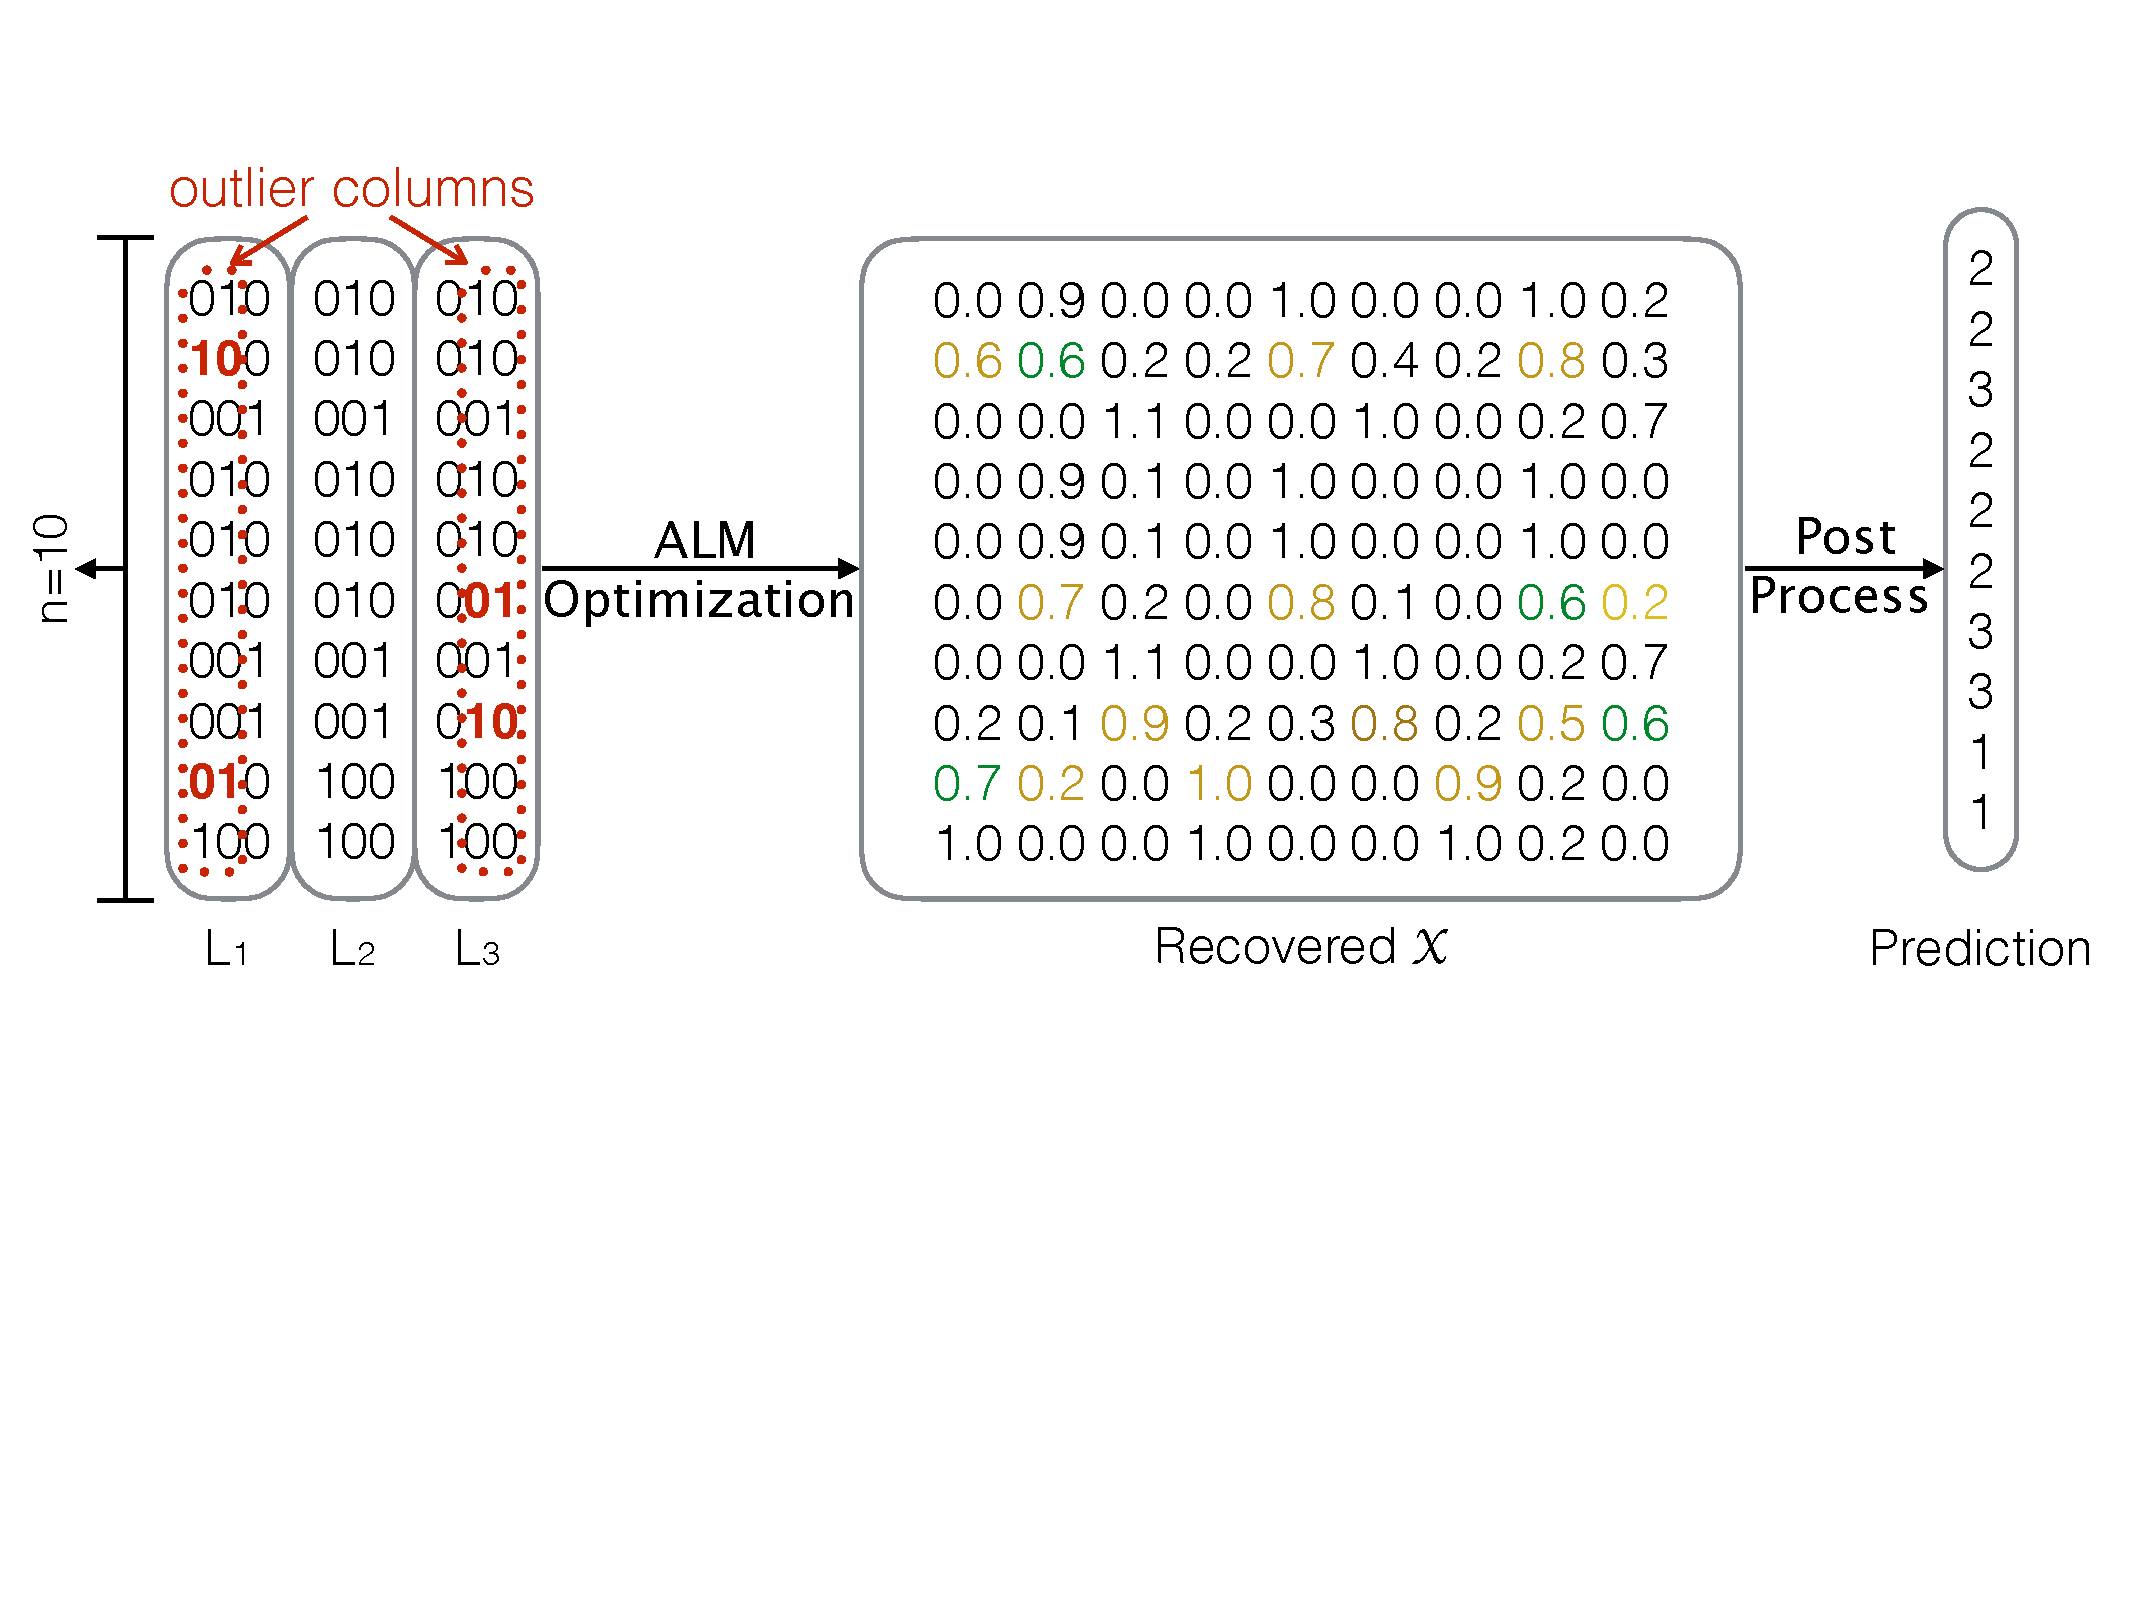
\includegraphics[width=0.45\textwidth]{resource/frame_work.pdf}
\caption{something}\label{fig:framework}
\end{figure}


\subsection{ALM Optimization}
Most existing matrix factorization optimization methods only consider smooth loss functions, but the $\ell_{1,2}$ loss in Problem~(\ref{eq:mf_l21}) is nonsmooth.
We apply ALM to optimize the nonsmooth objective function efficiently, desccribed as bellow: 

By introducing a new variable $\bE = \bL - \bX$, we can develop Problem~(\ref{eq:mf_l21}) as below:

\begin{align}\label{eq:mf_l21_constrained}
  \min_{\bE, \bX} ~&~ || \bE ||_{1,2}   \nonumber \\
  \st             ~&~ \bE = \bL - \bX   \nonumber \\
                  ~&~ \bX = \bU \bV,~\bU \in \dsR^{N \times k},~\bV \in \dsR^{k \times MK}
\end{align}
The augmented Lagrangian function of Problem~(\ref{eq:mf_l21}) is as below
\begin{align}\label{eq:lagrangian_l21}
  \calL = & || \bE ||_{1,2} + \langle \blambda, \bL - \bX - \bE \rangle + \frac{\mu}{2} || \bL - \bX - \bE ||_F^2
\end{align}
\noindent
where $\bX = \bU \bV$,
and $\blambda \in \dsR^{MK \times N}$ are the Lagrangian multipliers (or dual variables).
Then we could update $\bX$ and $\bE$ alternatively.


Specifically, to update $\bX$, we consider the following problem:
\begin{align}\label{eq:problem_X}
  \min_{\bX} ~&~ \langle \blambda, \bL - \bX - \bE \rangle + \frac{\mu}{2} || \bL - \bX - \bE ||_F^2  \nonumber  \\
  \st        ~&~ \bX = \bU \bV,~\bU \in \dsR^{N \times k},~\bV \in \dsR^{k \times MK}   .
\end{align}
Problem~(\ref{eq:problem_X}) includes a smooth loss function w.r.t. $\bX$, thus can be solved by a standard matrix factorization method, such as~\cite{yanijcai2015scalable,tanicml2014riemannian,vandereyckensiamjo2013low}.


Problem~(\ref{eq:problem_X}) can also be rewritten as below
\begin{align}\label{eq:problem_X2}
  \min_{\bX} ~&~ \frac{\mu}{2} \Big( || \bL - \bX - \bE ||_F^2 + \frac{2}{\mu} \langle \blambda, \bL - \bX - \bE \rangle + \frac{|| \blambda ||_F^2}{\mu^2} \Big)    \nonumber   \\
             ~&~ - \frac{\mu}{2} \frac{|| \blambda ||_F^2}{\mu^2}   \nonumber \\
  \st.       ~&~ \bX = \bU \bV,~\bU \in \dsR^{N \times k},~\bV \in \dsR^{k \times MK}   .
\end{align}
\noindent
We can obtain the final problem w.r.t. $\bX$:
\begin{align}\label{eq:problem_X3}
  \min_{\bX} ~&~ || \bL - \bX - \bE + \frac{\blambda}{\mu} ||_F^2   \nonumber \\
  \st        ~&~ \bX = \bU \bV,~\bU \in \dsR^{N \times k},~\bV \in \dsR^{k \times MK}   .
\end{align}
\noindent
There are a number of optimization algorithms for Problem~(\ref{eq:problem_X3}), such as LRGeomCG\footnote{\yanred{Code available at~\url{http://www.unige.ch/math/vandereycken/matrix_completion.html}}}.




To update $\bE$, we consider the following problem:
\begin{align}\label{eq:problem_E}
  \yanred{
  \min_{\bE} ~ || \bE ||_{1,2} + \langle \blambda, \bL - \bX - \bE \rangle + \frac{\mu}{2} || \bL - \bX - \bE ||_F^2   .
  }
\end{align}
\noindent
Similarly, we could reformulate the above problem as below:
\begin{align}\label{eq:problem_E2}
  \min_{\bE} & \frac{2}{\mu} || \bE ||_{1,2} + || \bL - \bX - \bE + \frac{\blambda}{\mu} ||_F^2    .
\end{align}
\noindent
Let $\bY = \bL - \bX + \frac{\blambda}{\mu}$.
The above problem can be efficiently solved by the following column-wise soft-thresholding operator:
\begin{align}\label{eq:column_wise_soft_thresholding}
  \bE_{i} = \calS_{\alpha}(\bY_{i}) = \left\{
    \begin{aligned}
      & \zerocolumn,~\text{if}~ ||\bY_{i}||_2 \leq \alpha   \\
      & \bY_{i} - \frac{\alpha \bY_{i}}{|| \bY_{i} ||_2},~\text{otherwise,}
    \end{aligned}
    \right.
\end{align}
\noindent
where $\bE_{i}$ and $\bY_{i}$ denote the $i$-th column of $\bE$ and $\bY$,
and $\alpha = \frac{2}{\mu}$.



We summarize the proposed algorithm for Problem~(\ref{eq:mf_l21_constrained}) in Algorithm~\
\begin{algorithm}[h!]
\begin{algorithmic}
\STATE Initialize $\rho > 1$, $t = 0$, $\blambda^{(t)} = 0$, and $\mu^{(t)} > 0$.

\STATE 1: Obtain $\bX^{(t)}$ by solving Problem~(\ref{eq:problem_X3}) via LRGeomCG.

\STATE 2: Obtain $\bE^{(t)}$ by column-wise soft-thresholding~(\ref{eq:column_wise_soft_thresholding}).

\STATE 2: $\blambda^{(t+1)} = \blambda^{(t)} + \mu^{(t)} (\bL - \bX^{(t+1)} - \bE^{(t+1)})$.

\STATE 3: $\mu^{(t+1)} = \rho \mu^{(t)}$.

\STATE 4: t = t + 1.

\STATE 5: Go to step 1 until convergence.

\end{algorithmic}
\caption{The ALM algorithm for Problem~(\ref{eq:mf_l21_constrained})} \label{Alg:overview_alm}
\end{algorithm}

\subsection{Final Post Process}
As we recover the low rank matrix X from the label assisnment matrix L. Intuitively, there is two possible way to get our final fusion results from X. Although L is a 01 matrix obtain by hard label, we could treat it as a soft score matrix, which the position of highest score represent the most possible label predicted by classifiers. X is an approximation of L, we can simply consider X as a soft score matrix, which fix the outliers from L. Two possible post way to processing X are described as bellow:
\begin{itemize}
  \item Average the score matrixs, each of which is a subset of X, the j-th matrix is from (j*k-k+1)-th colum to (j*k)-th colum of X. Then we got $X^*$, a N*K score matrix. we make the position of the highest value in each rows as the predicted label of the i-th instance.
  \item Seprate X into M matrixs $Y_j$, the i-th colum of $Y_j$ the (j*K+i)-th colum. For each matrix $Y_j$, we obtain a column vector by selecting the index of the highest score in each row. Then we use voting from M index matrix to select the final label.
\end{itemize}
According to the experiments, the first strategy outperform than the second one, we choose the first one as our final post process of fusion method.

\iffalse
\section{An Option on Loss Function: Max Margin}
In fact, the assignments $\bL$ contains only $0/1$ values (discrete ordinal values).
This fits the setting in~\cite{yanijcai2015scalable} very much.
It could be a contribution, since maximum margin loss achieves better performance on discrete ordinal values.
\yanred{Note: we may leave this extension as a journal?}

\section{Another Option on Loss Function: $\ell_{1,2}$ to $\ell_1$ loss}
$\ell_{1,2}$ loss could be difficult to optimize.
A simple way is to replace $\ell_{1,2}$ to $\ell_1$, which would be much easier.
\fi


\section{Experiments}
We visualize the results of our approach on one synthetic and evaluate the perfomance on five publicly available datasets : UCF101 human action dataset~\cite{soomro2012ucf101}, Cifar10~\cite{krizhevsky2009learning} dataset, PASCAL VOC’07~\cite{pascal-voc-2007}, Oxford Flower 17~\cite{nilsback2006visual} and Pascal Sentences dataset.
In UCF101 dataset, features are extracted from `fc6' layer of C3D model\cite{tran2015learning}, `pool5/7x7\_s1' layer from GoogleNet model\cite{szegedy2015going}, `pool5' layer of Residual Network model~\cite{he2015deep}, `fc6' layer of AlexNet,CaffeNet~\cite{krizhevsky2012imagenet} and Two-Stream Convolutional Networks~\cite{simonyan2014two}. Given a video, we sample 25 frames with equal temporal spacing between them as described in \cite{simonyan2014two} volumes for C3D). Following the same produce in \cite{tran2015learning} and \cite{simonyan2014two}, the features for the whole video are then calculated by averaging the features across the sampled frames.
In Cifar10 dataset, features are extracted from `global\_pool' layer of the ResnNt-20,32,44,56,110 models\cite{he2015deep} and pre-activation ResNet-20,32,44,56,110,164 models\cite{he2016identity}.
In all other dataset, features are extracted among `fc6' layer of VGG network~\cite{chatfield2014return} and AlexNet network~\cite{krizhevsky2012imagenet}, `pool5/7x7\_s1' layer from GoogleNet network~\cite{szegedy2015going}, `pool5' layer of Residual network~\cite{he2015deep}.
To be noted, all our cnn features are extracted using Caffe\cite{jia2014caffe}, a deep learning framework.

LIBLINEAR\cite{fan2008liblinear} is adopted for our classification toolbox, the confidence scores are generated from the outputs of LIBLINEAR. Then we put the confidence scores as the input into our alogrithm.

Five state-of-the-art fusion methods are compared with our proposed alogrithm : (1)Average Score Fusion(ASF), we directly average the confidence scores predicted by classifiers. We use $L_2$ norm on each classifiers for normalization. (2)Multiple Kernel Learning (MKL),  MKL learn a weight w for each classifiers, the final score are obtained from function $f(s)=w^{T}s, \sum w = 1$. We use liblinear-mkl\footnote{\url{http://www.csie.ntu.edu.tw/~b95028/software/liblinear-mkl/} ; \url{https://github.com/minghen/liblinear-mkl}} to train out MKL model. (3)Robust Convex Ensemble Clustering (RCEC)\cite{gaoijcai2016robust} (4)Feature Weighting via Optimal Thresholding(FWOT)\cite{xuiccv2013feature}. The author propse a method to learn thresholding, smoothing parameters and weights in a joint framework to combine prediction confidence scores of different features. (5)LPBoost\cite{gehler2009feature}. In this method, a variant linear combination are applied to multiple classifiers.

The parameter $\mu$ are selected from {0.1, 1, 5, 10}, $\rho$ are select from {1.01, 1.05, 1.1} in all our experiments. For SVM, we use the default parameters set in the LIBLINEAR.

\subsection{Synthetic Experiments}

In synthetic experiments, we set N = 320, M = 15, K = 20, randomly generate N instances with K kinds of labels. We randomly change 30\% instances' labels, repeat M times to get M classifiers' results. By appling our proposed alogrithm to this synthetic dataset, we visualize the results in Figure \ref{fig:ensemble_cluster}. Each subfigure contrains $N\times M$ small narrow blocks, which visualized in diverse colors according to their different label. The first picture~\ref{subfig:gt_pdf}, show the ground truth and copied M times. And M noised classifiers' results are pictured as~\ref{subfig:er_pdf}. After we recover the low rank matrix from the noised matrix by using ORLF late fusion method, we visualize it as~\ref{subfig:er_pdf}.



\begin{figure}[htp]
\center
    \subfigure[Ground Truth]{
    \label{subfig:gt_pdf}
    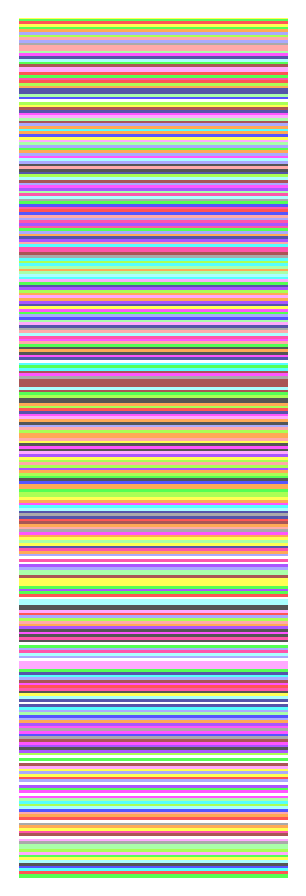
\includegraphics[width=0.14\textwidth]{resource/ground_truth.eps}
    }
    \subfigure[Random Noise]{
    \label{subfig:er_pdf}
    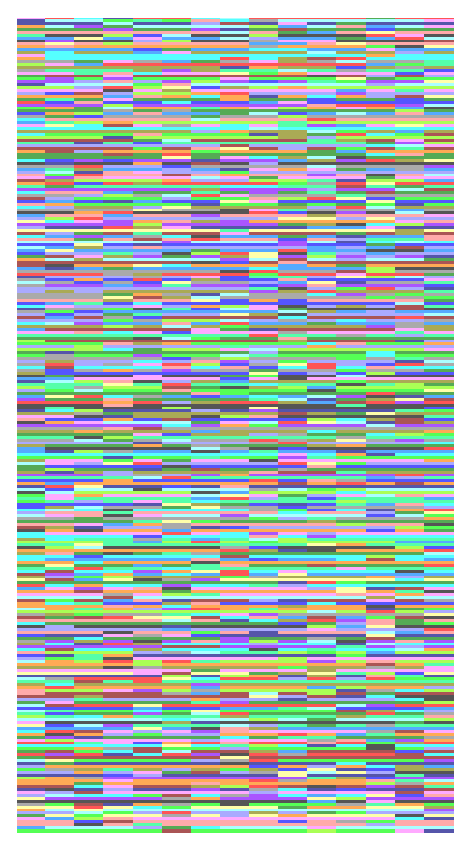
\includegraphics[width=0.14\textwidth]{resource/random_error.eps}
    }
    \subfigure[Outlier Reject]{
    \label{subfig:re_pdf}
    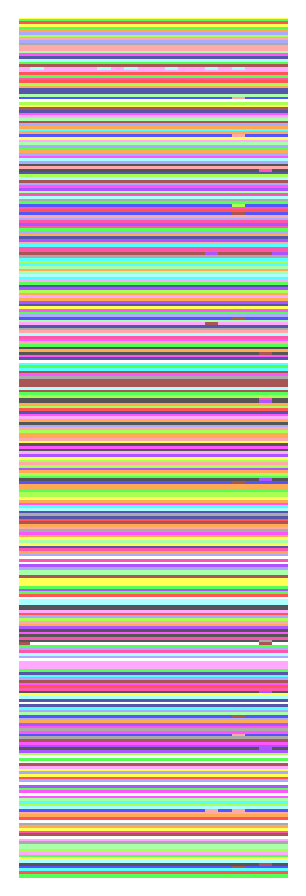
\includegraphics[width=0.14\textwidth]{resource/recover.eps}
    }
    \caption{visualized results of the synthetic dataset} \label{fig:ensemble_cluster}
\end{figure}


\iffalse
%We perform two experiments to show the effectiveness of the proposed outlier label pruning method.
%The first experiment is image classification with multiple features.
%The second experiment is ensemble classification.
%By these two experiments, we aim to demonstrate that our method is able to effectively remove the anomalous labels from the class indicator matrix, and thus improve the fusion performance of classification.
\fi

\subsection{Experiment on UCF 101 dataset}
For action recognition, we present our results on UCF 101 dataset\cite{soomro2012ucf101}. UCF101 contains 13320 videos collected from YouTube, categoried into 101 human action classes. We use the official split1 described in \cite{soomro2012ucf101}, which have 9573 training videos 3783 testing videos. As mentioned above, fives features are provided from the state of the art deep convolution networks, 4096 demitions features in `fc6' layer from C3D, 1028 demitions features in `pool5/7x7\_s1' layer from  GoogleNet, 2048 demitions features in `pool5' layer of ResNet-152, 4096 demitions features in `fc6' layer in Spatial and Temporal Net. All models used in UCF-101 are published by their authors.

We use liblinear to train seperate classifiers on each features with the default parameters in liblinear. By appling trained classifiers on test data, we can obtain 5 * 20 confidence score for each video. After emsenable fusion, we choose the class with highest confidence score as our predicted class. Results are shown in \ref{table:ucf101}, in which we illustrate the performance of the best single classifier and compare several fusion method.

\begin{table}[h]\small
\centering
\label{table:ucf101}
\begin{tabular}{c|c}
\hline
Method & Mean Accuracy(\%) \\\hline
SVM on Temporal Net Features & 86.2\% \\\hline
ASF &  86.8\% \\
MKL &  000 \\
RCEC &  000 \\
FWOT &  000 \\
LPBoost &  000 \\\hline
Ours &  000 \\
\hline
\end{tabular}
\caption{Mean Accuracy on UCF101 dataset for best single model and six fusion methods}
\end{table}




\subsection{Experiment on PASCAL VOC 2007 dataset}
PASCAL VOC 2007 is a dataset for object detection and image classification. For our experiment we only use the image level annotation information. Since each image may contain more than one label, we filter the multilabel images. Using the offical split provided by \cite{pascal-voc-2007}, we have 2954 trainval images and 3192 test images with 20 classes after filtration. We extract features from AlexNet,VGG,GoogleNet,ResNet, totally seven diffierent CNN features(AlexNet for alexnet and caffenet, VGG for VGG16 and VGG19, ResNet for ResNet50 and ResNet101).

After the procesure of classification and fusion, we got the results as \ref{table:voc}. Since in PASCAL VOC 2007 dataset, more classifiers are utilized than UCF101, it's clear that our method achieve significant improvement than single model and a slight improvement than other fusion algorithm.

\begin{table}[!h]\scriptsize
\centering
\label{table:voc}
\begin{tabular}{c|c|c|c}
\hline
Method            & Mean Accuracy & Classification Time(s)& Fusion Time \\\hline
Best Single Model & 88.44\%       &  2.347                &      0    \\\hline
ASF               & 88.69\%       &  10.2347              &    0.008   \\ % Average
MKL               &     0 & 00 & 0 \\
RCEC              &     0 & 0 & 000 \\
FWOT              &     0 & 0 & 000 \\
LPBoost           &     0 & 0 & 000 \\\hline
Ours              & 88.78\%       & 10.2347               & 9.918 \\
\hline
\end{tabular}
\caption{Accuracy and Time cost on VOC2007 dataset}
\end{table}


\subsection{Experiment on Cifar10 dataset}
In CIFAR-10 dataset, totally 60000 32x32 colour pictures are categoried into 10 classes, with 6000 pictures per class. There are 50000 training data and 10000 testing data. Fourteen CNN features are extracted from multiple state of the art models for training svm. These features are `global\_pool' layers' features of ResNet-20,32,44,56,110~\cite{he2015deep} and pre-activation ResNet-20,32,44,56,110,164~\cite{he2016identity},  `pool3' layer's features of cifar10\_full model described in caffe example prototxt\footnote{\url{https://github.com/BVLC/caffe/blob/master/examples/cifar10/cifar10_full.prototxt}} and `global\_pool' layers' features from two modified network from~\cite{szegedy2015going,chatfield2014return}. This experiments show the ability of our ORLF to handle large scale data.\yanred{(how to say)}

As we have 50000 training data and 10000 testing data, FWOT~\cite{xuiccv2013feature} has one step to deal with N*N matrixes, which are excessive to train~(more than one day) and LPBoost~\cite{gehler2009feature} need to create a $NK\times N$ constraint matrix linear programming solvers\footnote{The author use the MOSEK interior-point solver, see www.mosek.com.}, which occupies too much memory and still consumes long time to train. We use `-s 2' parameters in liblinear to speedup training training process. Results of other contrast algorithms are shown on \ref{table:cifar10}


\begin{table}[h]\scriptsize
\centering
\label{table:cifar10}
\begin{tabular}{c|c|c}
\hline
Method & Mean Accuracy(\%) & Classification Time + Fusion Time(s)\\\hline
ASF &  94.21\% & 55.6 + 0.02 \\
MKL &  94.15\% & 865.09 \\
RCEC &  94.87\% & 55.6 + 3.5 \\
FWOT &  - & - \\
LPBoost & - & - \\\hline
Ours &  95.05\% & 55.6 + 32.1 \\
\hline
\end{tabular}
\caption{Accuracy and Time cost on cifar10 dataset}
\end{table}



\subsection{Experiment on Oxford Flowers}
Oxford Flowers 17 dataset~\cite{nilsback2006visual} havs 17 flower categories with 80 images for each class. There are three predefined splits training set with 680 images, validation set with 340 images and testing set 340 images. 2048 dimetions `pool5' features from ResNet-50,101,152 proposed in \cite{he2015deep} and 4096 dimetions `fc6' features from CaffeNet,AlexNet proposed in \cite{krizhevsky2012imagenet} are used for linear SVM. The models are download from Caffe Model Zoo\footnote{\url{https://github.com/BVLC/caffe/wiki/Model-Zoo}}, with no finetuning on the current dataset.

We use the predefined training set and validation set as our training data, trained on liblinear with default parameters. For LPBoost Methods, we use 5 fold cross validation to select the best hyperparmeter $\nu$. 
Results are shown in \ref{table:flower17}


\begin{table}[h]\scriptsize
\centering
\label{table:flower17}
\begin{tabular}{c|c|c|c}
\hline
Method & Split 1 & Split 2 & Split 3\\\hline
ASF &  97.94\% & 0 & 0 \\
MKL &  000 & 0 & 0 \\
RCEC &  000 & 0 & 0 \\
FWOT &  000 & 0 & 0 \\
LPBoost & 97.94\% & 0 & 0 \\\hline
Ours &  98.24\% & 0 & 0 \\
\hline
\end{tabular}
\caption{Accuracy on Three Official Split}
\end{table}

\begin{quote}
\begin{small}
  \bibliographystyle{aaai}
  \bibliography{ensemble_clustering}
\end{small}
\end{quote}

\end{document}
